%! Author = tedro
%! Date = 23.03.21

% Preamble
\documentclass[a4paper, 11pt]{article}

% Packages
\usepackage[utf8]{inputenc}
\usepackage[czech]{babel}
\usepackage[left = 2cm, top = 3cm, total={17cm, 24cm}]{geometry}
\usepackage{amsmath}
\usepackage{times}
\usepackage{array}
\usepackage{multirow}
\usepackage[linesnumbered, longend, ruled, czech, noline]{algorithm2e}
\usepackage{graphicx}
\usepackage{lscape}
\usepackage{setspace}
\usepackage{hyperref}

% Document
\begin{document}
  \begin{titlepage}
    \begin{center}
      \Huge
      \textsc{Vysoké učení technické v~Brně} \\
      \huge\textsc{Fakulta informačních technologií} \\
      \vspace{\stretch{0.382}}
      \LARGE
      Typografie a publikování\,--\,3. projekt\\
      \Huge
      Tabulky a obrázky\\
      \vspace{\stretch{0.618}}
    \end{center}
    {\Large 23. března 2021\hfill
    Patrik Skaloš}
  \end{titlepage}

  \section{Úvodní strana}
  Název práce umístěte do zlatého řezu a nezapomeňte uvést dnešní datum a vaše
  jméno a příjmení.

  \section{Tabulky}
  Pro sázení tabulek můžeme použít buď prostředí\texttt{ tabbing }nebo
  prostředí\texttt{ tabular}.

  \subsection{Prostředí\texttt{ tabbing }}
  Při použití\texttt{ tabbing }vypadá tabulka následovně:
  \begin{tabbing}
    Vodní melouny \quad \= \textbf{Cena} \quad \= \kill
    \textbf{Ovoce} \> \textbf{Cena} \> \textbf{Množství} \\
    Jablka \> 25,90 \> 3 kg \\
    Hrušky \> 27,40 \> 2,5 kg \\
    Vodní melouny \> 35,-- \> 1 kus \\
  \end{tabbing}
  Toto prostředí se dá také použít pro sázení algoritmů, ovšem vhodnější je
  použít prostředí\texttt{ algorithm }nebo\texttt{ algorithm2e }(viz sekce \ref{algo}).

  \subsection{Prostředí\texttt{ tabular}}
  Další možností, jak vytvořit tabulku, je použít prostředí\texttt{ tabular}.
  Tabulky pak budou vypadat
  takto\footnote{Kdyby byl problem s\texttt{ cline,} zkuste se podívat třeba sem:
  \href{http://www.abclinuxu.cz/tex/poradna/show/325037.}{http://www.abclinuxu.cz/tex/poradna/show/325037}.}:
  \bigskip
  \begin{table}[h]
    \centering
    \catcode`\-=12
    \begin{tabular}{|l|l|l|}
      \hline
      \multirow[b]{2}{*}{\textbf{Měna}} &
        \multicolumn{2}{c|}{\textbf{Cena}} \\ \cline{2-3}
      & \textbf{nákup} & \textbf{prodej} \\
      \hline
      EUR & 25,227 & 26,943 \\
      \hline
      GBP & 29,368 & 31,492 \\
      \hline
      USD & 21,260 & 22,661 \\
      \hline
    \end{tabular}
    \caption{Tabulka kurzů k dnešnímu dni}
    \label{tab1}
  \end{table}
  \bigskip
  \begin{table}[h]
    \centering
    \catcode`\-=12
    \begin{tabular}{|c|c|}
      \hline
      $A$ & $\neg A$ \\
      \hline
      \textbf{P} & N \\
      \hline
      \textbf{O} & O \\
      \hline
      \textbf{X} & X \\
      \hline
      \textbf{N} & P \\
      \hline
    \end{tabular}
    \begin{tabular}{|c|c|c|c|c|c|}
      \hline
      \multicolumn{2}{|c|}{\multirow{2}{*}{$A \wedge B$}} & \multicolumn{4}{c|}{$B$} \\
        \cline{3-6}
      \multicolumn{2}{|c|}{} & \textbf{P} & \textbf{O} & \textbf{X} & \textbf{N} \\
      \hline
      \multirow{4}{*}{$A$} & \textbf{P} & P & O & X & N \\ \cline{2-6}
                           & \textbf{O} & O & O & N & N \\ \cline{2-6}
                           & \textbf{X} & X & N & X & N \\ \cline{2-6}
                           & \textbf{N} & N & N & N & N \\ \cline{2-6}
      \hline
    \end{tabular}
    \begin{tabular}{|c|c|c|c|c|c|}
      \hline
      \multicolumn{2}{|c|}{\multirow{2}{*}{$A \vee B$}} & \multicolumn{4}{c|}{$B$} \\
      \cline{3-6}
      \multicolumn{2}{|c|}{} & \textbf{P} & \textbf{O} & \textbf{X} & \textbf{N} \\
      \hline
      \multirow{4}{*}{$A$} & \textbf{P} & P & P & P & P \\ \cline{2-6}
                           & \textbf{O} & P & O & P & O \\ \cline{2-6}
                           & \textbf{X} & P & P & X & X \\ \cline{2-6}
                           & \textbf{N} & P & O & X & N \\ \cline{2-6}
      \hline
    \end{tabular}
    \begin{tabular}{|c|c|c|c|c|c|}
      \hline
      \multicolumn{2}{|c|}{\multirow{2}{*}{$A \rightarrow B$}} & \multicolumn{4}{c|}{$B$} \\
      \cline{3-6}
      \multicolumn{2}{|c|}{} & \textbf{P} & \textbf{O} & \textbf{X} & \textbf{N} \\
      \hline
      \multirow{4}{*}{$A$} & \textbf{P} & P & O & X & N \\ \cline{2-6}
                           & \textbf{O} & P & O & P & O \\ \cline{2-6}
                           & \textbf{X} & P & P & X & X \\ \cline{2-6}
                           & \textbf{N} & P & P & P & P \\ \cline{2-6}
      \hline
    \end{tabular}
    \caption{Protože Kleeneho trojhodnotová logika už je \uv{zastaralá}, uvádíme
    si zde příklad čtyřhodnotové logiky}
    \label{tab2}
  \end{table}
  \bigskip

  \pagebreak

  \section{Algoritmy}
  \label{algo}
  Pokud budeme chtít vysázet algoritmus, můžeme použít
  prostředí\texttt{ algorithm\footnote{
    Pro nápovědu, jak zacházet s prostředím\texttt{ algorithm,} můžeme
    zkusit tuhle stránku:\\
    \href{http://ftp.cstug.cz/pub/tex/CTAN/macros/latex/contrib/algorithms/algorithms.pdf}
    {http://ftp.cstug.cz/pub/tex/CTAN/macros/latex/contrib/algorithms/algorithms.pdf}.
  } } nebo\texttt{ algorithm2e\footnote{
    Pro\texttt{ algorithm2e }zase tuhle: 
    \href{http://ftp.cstug.cz/pub/tex/CTAN/macros/latex/contrib/algorithm2e/doc/algorithm2e.pdf}
    {http://ftp.cstug.cz/pub/tex/CTAN/macros/latex/contrib/algorithm2e/doc/algorithm2e.pdf}.
  }}. Příklad použití prostředí\texttt{ algorithm2e }viz Algoritmus \ref{algo1}.
  \vspace{0.95em}
  \begin{algorithm}[h]
    \label{algo1}
    \caption{\textsc{Fast}SLAM}
    \KwIn{ $(X_{t-1}, u_t, z_t)$}
    \KwOut{ $X_t$}
    \Indp\Indpp\Indpp
    \SetNlSty{}{}{:}
    \SetNlSkip{-1.2em}
    \SetAlgoNlRelativeSize{-1}
    \medskip
    $\overline{X_t} = X_t = 0$ \\
    \setstretch{0.87}
    \For{$k = 1$ \textnormal{to} $M$}{
      $x_t^{[k]} = \emph{sample\_motion\_model}(u_t, x_{t-1}^{[k]})$ \\
      $\omega_t^{[k]} = \emph{measurement\_model}(z_t, x_t^{[k]}, m_{t-1})$ \\
      $m_t^{[k]} = updated\_occupancy\_grid(z_t, x_t^{[k]}, m_{t-1}^{[k]})$ \\
      $\overline{X_t} = \overline{X_t} + \langle x_x^{[m]}, \omega_t^{[m]} \rangle$ 
    }
    \For{$k = 1$ \textnormal{to} $M$}{
      draw $i$ with probability $\approx \omega_t^{[i]}$ \\
      add $\langle x_x^{[k]}, m_t^{[k]} \rangle$ to $X_t$ \\
    }
    \Return{ $X_t$}
    %TODO
  \end{algorithm}

  \section{Obrázky}
  Do našich článků můžeme samozřejmě vkládat obrázky. Pokud je obrázkem 
  fotografie, můžeme klidně použít bitmapový soubor. Pokud by to ale
  mělo být nějaké schéma nebo něco podobného, je dobrým zvykem takovýto
  obrázek vytvořit vektorově.

  \begin{figure}[h]
    \centering
    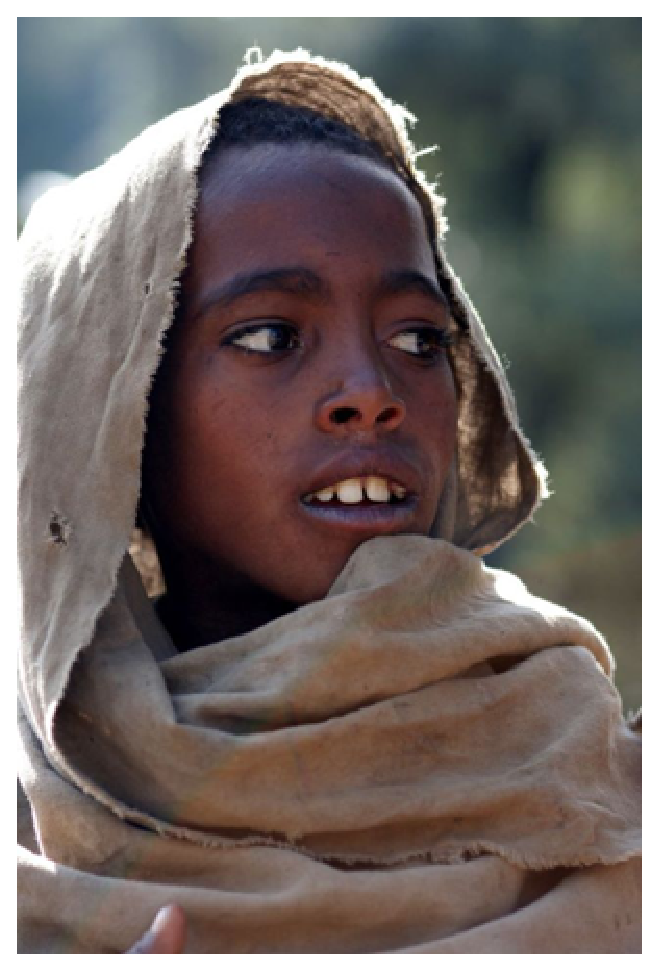
\includegraphics[width=4.25cm]{./src/etiopan.eps}\,\reflectbox{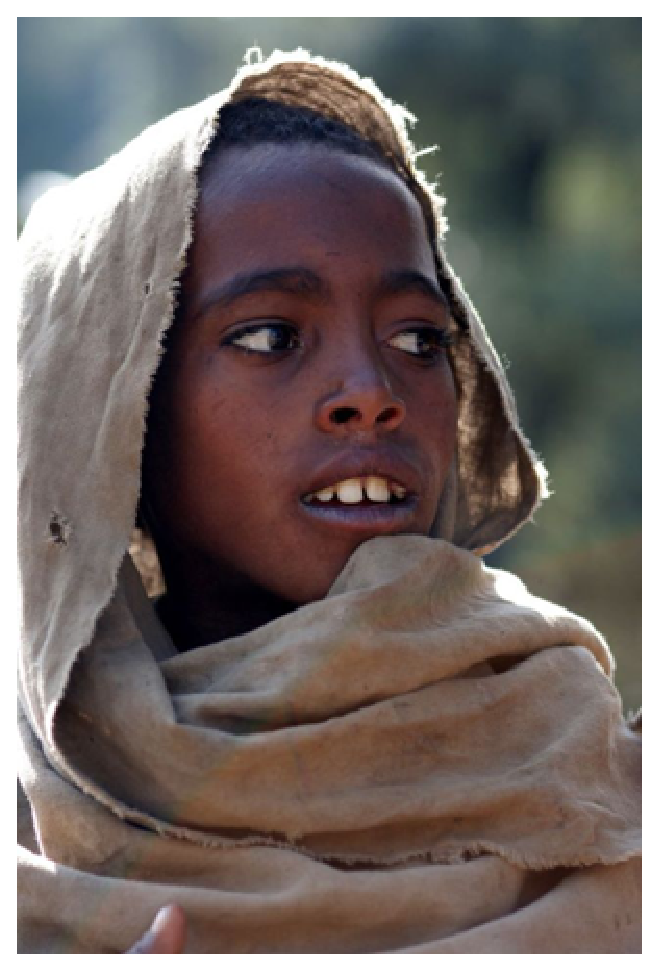
\includegraphics[width=4.25cm]{./src/etiopan.eps}}
    \caption{Malý Etiopánek a jeho bratříček}
    \label{obr1}
  \end{figure}

  \newpage

  Rozdíl mezi vektorovým\,\dots
   
  \begin{figure}[h]
    \centering
    \scalebox{0.4}{
\includegraphics{src/oniisan.eps}}
    \caption{Vektorový obrázek}
    \label{obr2}
  \end{figure}

  \bigskip
  \noindent \dots\,a bitmapovým

  \begin{figure}[h]
    \centering
    \scalebox{0.6}{
\includegraphics{src/oniisan2.eps}}
    \caption{Bitmapový obrázek}
    \label{obr3}
  \end{figure}

  \bigskip
  \noindent se projeví například při zvětšení.

  Odkazy (nejen ty) na obrázky \ref{obr1}, \ref{obr2} a \ref{obr3}, na tabulky 
  \ref{tab1} a \ref{tab2} a také na 
  algoritmus \ref{algo1} jsou udělány pomocí křížových odkazů. Pak je ovšem
  potřeba zdrojový soubor přeložit dvakrát.

  Vektorové obrázky lze vytvořit i přímo v \LaTeX{u}, například pomocí
  prostředí\texttt{ picture.}

  \newpage

  \begin{landscape}
    \begin{figure}[h]
      \centering
      \setlength{\unitlength}{1cm}
      \thicklines
      \begin{picture}(20, 10.8)
        \put(0, 0){\framebox(20, 10){}}

        %Sun
        \put(2,8){\circle{1}}
        \put(2.75, 8){\line(1, 0){1}}
        \put(2.5, 8.5){\line(1, 1){0.75}}
        \put(2, 8.75){\line(0, 1){1}}
        \put(1.5, 8.5){\line(-1, 1){0.75}}
        \put(1.25, 8){\line(-1, 0){1}}
        \put(1.5, 7.5){\line(-1, -1){0.75}}
        \put(2, 7.25){\line(0, -1){1}}
        \put(2.5, 7.5){\line(1, -1){0.75}}

        %House
        \put(5, 0){\line(0, 1){8}}
        \put(15, 0){\line(0, 1){8}}
        \put(5, 8){\line(5, 2){5}}
        \put(15, 8){\line(-5, 2){5}}

        %Windows
        \put(6.5, 7.5){\line(1, 0){2}}
        \put(6.5, 5.5){\line(0, 1){2}}
        \put(6.5, 5.5){\line(1, 0){2}}
        \put(8.5, 5.5){\line(0, 1){2}}
        \put(7.5, 5.5){\line(0, 1){2}}

        \put(11.5, 7.5){\line(1, 0){2}}
        \put(11.5, 5.5){\line(0, 1){2}}
        \put(11.5, 5.5){\line(1, 0){2}}
        \put(13.5, 5.5){\line(0, 1){2}}
        \put(12.5, 5.5){\line(0, 1){2}}

        %Garage
        \put(6, 0){\line(0, 1){3}}
        \put(6, 3){\line(1, 0){4}}
        \put(10, 0){\line(0, 1){3}}
        \put(7.9, 0.75){\line(1, 0){0.2}}

        %Door
        \put(12, 0){\line(0, 1){4}}
        \put(12, 4){\line(1, 0){2}}
        \put(14, 0){\line(0, 1){4}}
        \put(12.25, 2){\circle*{0.2}}
        \put(12.7, 3.25){\textbf{My}}

        %Postbox
        \put(17, 0){\line(0, 1){2}}
        \put(17.5, 0){\line(0, 1){2}}
        \put(16.75, 2){\line(1, 0){1}}
        \put(16.75, 2){\line(0, 1){0.5}}
        \put(17.75, 2){\line(0, 1){0.5}}
        \put(17.25, 2.5){\oval(1,1)[t]}
        \put(17, 2.25){\line(1, 0){0.5}}
        \put(17, 2.5){\textbf{My}}

      \end{picture}
      \caption{Vektorový obrázek domečku.}%TODO
  \end{figure}
\end{landscape}
\end{document}
